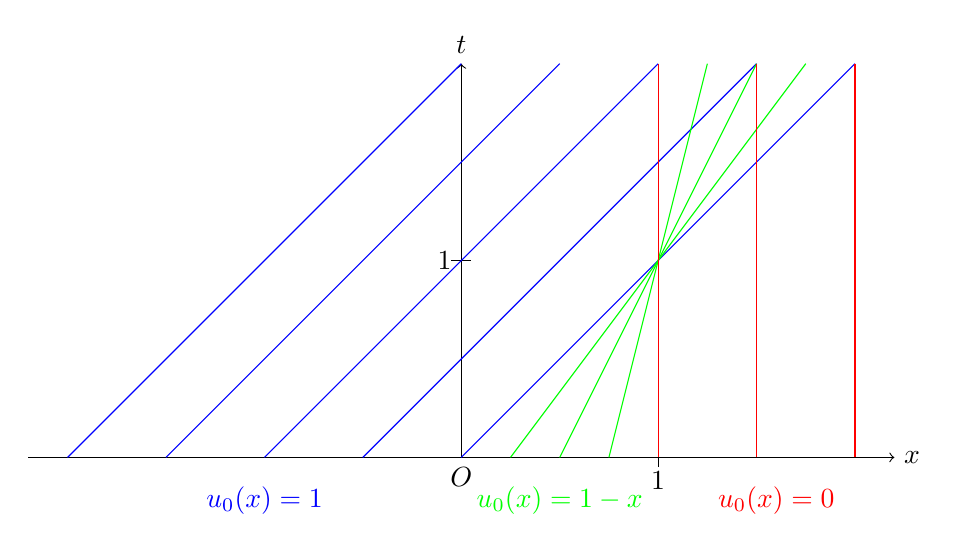
\begin{tikzpicture}[scale=2.5]
\draw[->] (-2.2,0) -- (2.2,0);
\draw (2.2,0) node[right] {$x$};
\draw[->] (0,0) -- (0,2);
\draw (0,2) node[above] {$t$};
\draw (0,0) node[below] {$O$};
\draw (1,-0.05) -- (1,0.05);
\draw (1,-0.025) node[below] {$1$};
\draw (-0.05,1) -- (0.05,1);
\draw (0,1) node[left] {$1$};

\draw[blue] (-2,0) -- (0,2);
\draw[blue] (-1.5,0) -- (0.5,2);
\draw[blue] (-1,0) -- (1,2);
\draw[blue] (-0.5,0) -- (1.5,2);
\draw[blue] (0,0) -- (2,2);
\draw[blue] (-1,-0.1) node[below] {$u_0(x)=1$};

\draw[green] (0.25,0) -- (1.75,2);
\draw[green] (0.5,0) -- (1.5,2);
\draw[green] (0.75,0) -- (1.25,2);
\draw[green] (0.5,-0.1) node[below] {$u_0(x)=1-x$};

\draw[red] (1,0) -- (1,2);
\draw[red] (1.5,0) -- (1.5,2);
\draw[red] (2,0) -- (2,2);
\draw[red] (1.6,-0.1) node[below] {$u_0(x)=0$};
\end{tikzpicture}